\documentclass[a4paper,11pt]{article}
% ---- graphiques
\usepackage[pdftex]{graphicx}

% for latex2html
\usepackage{html}

% for accents
\usepackage[latin1]{inputenc}

% ---- inclusion de codes
\usepackage{listings}
\lstset{showstringspaces=false,frame=trBL,frameround=tttt,tabsize=4,basicstyle=\tiny,breaklines=true,breakatwhitespace=true}
\lstdefinestyle{bash}{language=bash}
\lstdefinestyle{Perl}{language=Perl}
\lstdefinestyle{C++}{language=C++}
\lstdefinestyle{DTD}{language=XML}
\lstdefinestyle{XML}{language=XML,usekeywordsintag=false,markfirstintag=true}
%begin{latexonly}
\newcommand{\includecode}[2]{
\lstinputlisting[style=#1]{#2}
}
%end{latexonly}
\begin{htmlonly}
\newcommand{\includecode}[2]{  \htmladdnormallink{#2}{../../#2} }
\end{htmlonly}
%\lstnewenvironment{code}{}{}
\lstnewenvironment{code_bash}{\lstset{style=bash}}{}
\lstnewenvironment{code_perl}{\lstset{style=Perl}}{}
\lstnewenvironment{code_cpp}{\lstset{style=C++}}{}
\lstnewenvironment{code_dtd}{\lstset{style=DTD}}{}
\lstnewenvironment{code_xml}{\lstset{style=XML}}{}

\newcommand{\textcode}[1]{{\small {\tt #1}}}




\newcommand{\sofa}{SOFA }
\newcommand{\todo}[1]{}
\newcommand{\eg}{\textit{e.g.} }


% macros mathematiques
\newcommand{\ma}[1]{\ensuremath{\mathbf {#1}}}
\newcommand{\ve}[1]{\ensuremath{\mathbf {#1}}}

\usepackage{amsmath}
\usepackage{amsfonts}
\usepackage{amssymb}

% character styles
\newcommand{\bm}[1]{\ensuremath{\mathbf{{#1}}}}
\newcommand{\mcal}[1]{\mbox{$\mathcal #1$}} % rondes math
\newcommand{\bmcal}[1]{\mbox{\boldmath $\mathcal #1$}} % rondes grasses math
\newcommand{\ensemble}[1]{\mbox{$\mathbb{#1}$}}
\newcommand{\RRR}{\mbox{$\ensemble{R}^3$}} 


% d�finitions
\newcommand{\definition}[2]{\index{#1}{\bf #1}: #2}
\newcommand{\voc}[1]{\index{#1}#1}
\newcommand{\bvoc}[1]{\index{#1}{\bf #1}}

% misc
\newcommand{\EV}[1]{\stackrel{\rightarrow}{#1}}  % espace vectoriel
\newcommand{\EA}[1]{#1}                          % espace affine

% vectors, matrices
%\newcommand{\point}[1]{\mbox{$#1$}}          % un point
\newcommand{\point}[1]{\ensuremath{#1}}          % un point
\newcommand{\mat}[1]{\bm{#1}}         % matrice
\newcommand{\matnm}[3]{\bm{#1_{#2\times #3}}}  % matrice n lignes , m colonnes
\newcommand{\vect}[1]{\bm{#1}}        % vecteur 
%\newcommand{\vecf}[1]{\stackrel{\rightarrow}{#1}}  % vecteur avec fleche
\newcommand{\vecf}[1]{\mbox{$\overrightarrow{#1}$}}  % vecteur avec fleche
\newcommand{\ident}[1]{\bm{I_{#1}}}   % identit� en dimension n
\newcommand{\inv}[1]{#1^{-1}}         % matrice inverse
\newcommand{\psinv}[1]{#1^{+}}        % matrice pseudo-inverse
\newcommand{\transp}[1]{#1^T}         % transpos�e de 1
\newcommand{\trace}[1]{tr(#1)}        % trace
\newcommand{\deter}[1]{\mbox{$|#1|$}}       % determinant
\newcommand{\oppvec}[1]{\mbox{$\left( \vect {#1} \wedge \right)$}}  % operateur matriciel de produit vectoriel

% bases, reperes
\newcommand{\vecin}[2]{\mbox{${}^{#2}#1$}}    % vecteur 1 dans repere 2
\newcommand{\Base}[1]{\ensuremath{\mathcal B_{#1}}} % Symbole du repere 1
\newcommand{\chbase}[3]{\mbox{${}_{#2}^{#3}\mat{#1}$}}  % operateur 1 fait le passage de la base 3 vers la base 2
%\newcommand{\pchbase}[2]{\chbase{\mat{B}}{#1}{#2}}  % matrice de passage de la base 2 vers la base 1
\newcommand{\pchbase}[2]{\chbase{B}{#1}{#2}}  % matrice de passage de la base 2 vers la base 1
\newcommand{\Rep}[1]{\ensuremath{\mathcal R_{#1}}} % Symbole du repere 1
\newcommand{\rep}[1]{\Rep{#1}}                 % Symbole du repere 1
%\newcommand{\pchrep}[2]{\chbase{\mat{F}}{#1}{#2}}  % matrice de passage du repere 1 vers le repere 2, F comme Frame
\newcommand{\pchrep}[2]{\chbase{\bm{C}}{#1}{#2}}  % matrice de passage du repere 2 vers le repere 1

%% Operateur de passage du repere 1 par rapport a 2
%\newcommand{\ChgRep}[2]{\mbox{\boldmath $R_{#1}^{#2}$}}

% rotations	
%\newcommand{\rot}[2]{\mbox{$\mat{R}_{#1,#2}$}}      % rotation vectorielle
\newcommand{\rot}[2]{\ensuremath{\mat{R}_{#1,#2}}}      % rotation vectorielle
\newcommand{\rota}[3]{\mbox{$\mat{R}_{#1,#2,#3}$}}  % rotation affine

% translation
\newcommand{\trans}[2]{\mbox{$\chbase{\vect{t}}{#1}{#2}$}} % passage de #1 vers #2 par une translation, ou translation du repere #2 par rapport au repere #1

% vitesses et acc�l�rations
\newcommand{\VRep}[2]{\mbox{\boldmath $\dot R_{#1}^{#2}$}} % vitesse du repere 1 par rapport a 2 
%\newcommand{\Point}[2]{\mbox{\boldmath ${#1}^{#2}$}}  % Coordonnees d'un point 1 dans un repere 2
\newcommand{\Point}[2]{\mbox{$\vecin{\bm{#1}}{#2}$}}  % Coordonnees d'un point 1 dans un repere 2
\newcommand{\VPoint}[2]{\mbox{\boldmath ${\dot #1}_{/#2}$}} % Vitesse d'un point par rapport � un repere
\newcommand{\APoint}[2]{\mbox{\boldmath ${\ddot #1}_{/#2}$}} % Acceleration d'un point par rapport � un repere

% cinematique du solide
\newcommand{\derivedans}[2]{\mbox{$\dot{#1}^{(#2)}$}}  % derivee du vecteur 1 dans repere 2
\newcommand{\fixedans}[2]{\mbox{$#1_{\in #2}$}}        % vecteur 1 fixe dans repere 2
\newcommand{\vecom}{\mbox{$\bm{\Omega}$}}  % omega de 1 par rapport a 2
\newcommand{\vecrot}[2]{\mbox{$\vecom_{#1/#2}$}}  % omega de 1 par rapport a 2
\newcommand{\accrot}[2]{\mbox{$\dot{\vecom}_{#1/#2}$}}  % omega de 1 par rapport a 2
\newcommand{\vfdans}[3]{\mbox{$\vec V^{#2/#3}_{#1}$}}    % vitesse de 1 fixe dans 2 par rapport a 3
\newcommand{\afdans}[3]{\mbox{$\vec \Gamma^{#2/#3}_{#1}$}}    % acceleration de 1 fixe dans 2 par rapport a 3
\newcommand{\vmdans}[2]{\mbox{$\vec V^{/{#2}}_{#1}$}}    % vitesse de 1 mobile dans 2
\newcommand{\amdans}[2]{\mbox{$\vec \Gamma^{/#2}_{#1}$}}    % acceleration de 1 mobile dans 2

% chaines articulees
\newcommand{\liaison}[2]{\mbox{$\mathcal L_{#1,#2}$}}  % liaison du pere 1 vers fils 2 (et repere intermediaire)
\newcommand{\liaisonprime}[2]{\mbox{$\mathcal L'_{#1,#2}$}}  % deuxieme repere intermediaire de la liaison du pere 1 vers fils 2
\newcommand{\liaisonP}[2]{\mbox{$\mathcal L_{#1,#2}$}}  % Repere dans pere 1 de la liaison vers fils 2 
\newcommand{\liaisonC}[2]{\mbox{$\mathcal L'_{#1,#2}$}}  % Repere dans fils de la liaison du pere 1 vers fils 2 
%\newcommand{\transP}[2]{\pchrep{\liaisonP{#1}{#2}}{#1}}  % Matrice du repere dans pere de la liaison du pere 1 vers fils 2 
%\newcommand{\transC}[2]{\pchrep{\liaisonC{#1}{#2}}{#2}}  % Matrice du repere dans pere de la liaison du pere 1 vers fils 2 
%\newcommand{\transPC}[2]{\pchrep{\liaisonC{#1}{#2}}{\liaisonP{#1}{#2}}}  % matrice de passage entre repere liaison dans fils et repere de liaison dans pere
\newcommand{\transP}[2]{\chbase{C_p}{#2}{#1}}  % Matrice du repere dans pere de la liaison du pere 1 vers fils 2 
\newcommand{\transC}[2]{\chbase{C_c}{#2}{#1}}  % Matrice du repere dans pere de la liaison du pere 1 vers fils 2 
\newcommand{\transPC}[2]{\chbase{C_l}{#2}{#1}}  % matrice de passage entre repere liaison dans fils et repere de liaison dans pere
% \pchrep{fils}{pere} = \liaisonP{pere}{fils}\deplPC{pere}{fils}\liaisonC{pere}{fils}


\newcommand{\pctab  }{\hspace{0.15in}      }  % Pseudo-code indentation.
\newcommand{\code}[1]{ 
\begin{makeimage}
\begin{tabbing} \pctab \= \pctab \= \pctab \= \pctab \= \pctab \= \pctab \= \pctab \kill
#1
\end{tabbing}
\end{makeimage}
}
 % This file is in parent directory. Your TEXINPUTS environment variable must include .. to reach this file. Example: setenv TEXINPUTS ..:../..:${TEXINPUTS}

% ---- format de page A4
	\setlength{\textwidth }{16cm}	% largeur de ligne
	\setlength{\textheight}{23cm}   % hauteur du texte
	\setlength{\oddsidemargin}{0cm} % marge pages impaires
	\setlength{\evensidemargin}{0cm}% marge pages paires
	\setlength{\topmargin}{0cm} 	
	\setlength{\headheight}{14pt} 
	\setlength{\headsep}{0.5cm} 


% Title Page
\title{High Order Elements in Sofa}
%\author{The \sofa{} team}
\date{2014}
\author{Herv\'e Delingette\\ {\small INRIA M\'editerran\'ee, Sophia Antipolis, France}}





\begin{document} 
\maketitle
\section{High Order Tetrahedral Meshes}

\subsection{Introduction}

We define high order tetrahedral elements in their Bernstein / Bezier form rather than Hermite form. 
A high order tetrahedral mesh is defined by :

\begin{itemize}
	\item An underlying tetrahedral mesh $\mesh$ consisting of a set of {\em "tetrahedron vertices"} $\vertices$, edges $\edges$, triangles $\triangles$ and tetrahedra $\tetrahedra$. We write $\nvertices$, the number of "tetrahedron vertices", $\nedges$ the number of edges, $\ntriangles$ the number of triangles and $\ntetrahedra$ the number of tetrahedra. 
	\item A set of control points $\controls$
	\item A set of quadrivariate Bernstein polynomials  allowing to describe the value of a node anywhere on the mesh $\mesh$ 
\end{itemize}
%\section{Athapascan Interface Overview}
Athapascan is an interface to describe a data flow graph, composed by a set of tasks accessing data according to a given pattern. 
All the data to be inserted in the Data Flow must be of the type Shared<TYPE> where TYPE is the type of information we want to represent in the graph.
Tasks are created using a Fork primitive. Each time we create a now task we must specify the access mode for each parameter.

With this information Athapascan is able to link the tasks respecting the data access order.
Here is an example where we create a Shared variable, that is accessed by two tasks, one writing a value and another one that reads it.
\begin{verbatim}

class Task1{
	public:	
	void operator()(Shared_w<int> x){
		x.write(2);
		}
};
class Task2{
	public:	
	void operator()(Shared_rw<int> x){
		int & x1=x.access();
		x1++;
		}
};

class Task3{
	public:
	void operator()(Shared_r<int> x){
	    cout<<x.read()<<endl;
	    }
};


void main(){

	Shared<int> var1; //Create Var1
	Fork<Task1>()(var1); //Insert task 1 in the Graph
	Fork<Task2>()(var1);//insert task 2 in the Graph
	Fork<Task2>()(var1);//insert task 2 in the Graph
	Fork<Task3>()(var1);//insert task 3 in the Graph
	Sync(); //Execute the graph
}
\end{verbatim}

All the tasks inserted in a graph must be implemented as Functors. A Functor is a class that overloads the  operator(). When using Functors we are sure that none of the computation depends on class attributes, and all the  needed data is passed as parameter. The remote execution of this kind of task becomes easier, as we only need to transfer the Functors arguments.

A \textbf{ Shared\_r} represents a read only data. It must be accessed using the read() function, that returns a \textbf{const} reference to the data. A read/write argument is represented by a Shared\_rw, it is accessed by the access() function, that returns a pointer to the data which can be modified. A write only argument, Shared\_w, can only be written through the \textbf{write(}newValue\textbf{)} function, it ensures that there will be no reading in the object, as it doesn't returns a pointer to the data. 

There is also a cumulative write type, that allows to make parallel accumulative operations. It's not fully functional, but will be used on addForce Operations.

\section{Using Athapascan inside Sofa}
To create an Athapascan Graph in Sofa we need to specify the tasks we want to insert in the graph and execute in  parallel, and some Shared data, that are accessed by those tasks. 
\subsection{Shared Data}
To have Athapascan Shared types in Sofa, we have created new types to be used by multivectors, a VecCoordShared and a VecCoordDeriv. They are implemented as follows:

\begin{verbatim}
 typedef Shared<VecCoord> VecCoordShared;
 typedef Shared<VecDeriv> VecDerivShared;
\end{verbatim}

For compatibility reasons we conserved all the VecCoord and VecDeriv variables and created equivalent variables of type VecCoordShared and VecDerivShared. For example for a MechanicalObject we have \textbf{xSh} attribute that is used when executing the Athapascan implementation, and a \text{x} attribute that is used by the standard implementation. By the same way there are getX and getXSh object functions. There is also a getXfromSh and getVfromSh that can be used to access directly the data inside a Shared.  It only makes sense to access getXfromSh before and after the graph execution, as during the graph execution we have no guarantees on the consistency of this information.	

Shared versions of \textbf{Data} and \textbf{DataPtr} were created as \textbf{DataShared} \textbf{DataPtrShared}. They must be used when we have a Data that must  to be considered for the  data dependency  graph. Also it is useful to avoid large Data to be passed as value instead of reference. A task argument that is not a Shared is allways passed by copy, while a Shared type is allways passed as reference. A copy  of a Shared occurs only for network data transfer on remote calls.


In terms of topology, a high order tetrahedral mesh has more control points than tetrahedron vertices.
Below are examples of high order tetrahedral elements of various degree.
\begin{figure}[!htbp]
	\centering
    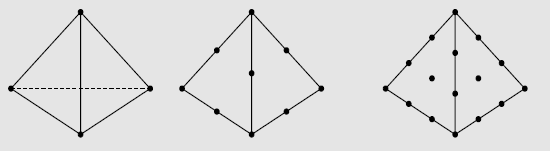
\includegraphics[width=0.80\textwidth]{HighOrderTetra}
	\caption{Linear ($\degree=1$), Quadratic ($\degree=2$) and Cubic ($\degree=3$) Tetrahedral Elements}
	\label{fig:LinearQuadraticAndCubicTetrahedralElements}
\end{figure}


\subsubsection{Number of Control Points}

If we write $\degree>0$ the degree (or order) of a tetrahedral element, then there are :

\begin{itemize}
	\item $\nvertices$ controls points that coincide with the {\em "tetrahedron vertices"}.
	\item $(\degree-1) \nedges$ if $\degree>1$ control points that are lying on edges. 
	\item $\frac{(\degree-1) (\degree-2) \ntriangles}{2}$ if $\degree>2$ control points that are lying on triangles. 
	\item $\frac{(\degree-1) (\degree-2) (\degree-3) \ntetrahedra}{6}$ if $\degree>3$ control points that are lying on tetrahedra. 
\end{itemize}

Thus the total number of control points are :
\[
\ncontrols=\nvertices+(\degree-1) \nedges+\frac{(\degree-1) (\degree-2) \ntriangles}{2}+\frac{(\degree-1) (\degree-2) (\degree-3) \ntetrahedra}{6}
\]
\subsubsection{Tetrahedron Bezier Indices}

We use specific notations of control points inside a tetrahedron which we call {\em Tetrahedron Bezier Indices} (TBI).
A TBI $p\in \naturalSet^{+}\times\naturalSet^{+}\times\naturalSet^{+}\times\naturalSet^{+}$ is a 4-plet of positive natural numbers that indicate their relative position in the high order element. 

Thus for an element of degree $\degree$, ${\mathbf p}=(i,j,k,l)$ is such that $|{\mathbf p}|=i+j+k+l=\degree$.  The four TBI $(\degree,0,0,0)$, $(0,\degree,0,0)$, $(0,0,\degree,0)$, $(0,0,0,\degree)$ coincides with the 4 tetrahedron vertices while $(0,i,0,j), i>0, j>0$ is lying on the edge linking the second and fourth vertex and   $(0,i,j,k), i>0, j>0, k>0$ is lying on the triangle opposite to the first vertex. We write $\control_{\mathbf p}$ the control point associated with indices $(i,j,k,l)$.

\subsubsection{Tetravariate Bernstein Polynomial}

The control points are used to define a parametric volume in space. The parameters are the barycentric coordinates $(r,s,t,u)$ such that $r+s+t+u=1$ and $0\leq r,s,t,u \leq 1$. The shape functions are the tetravariate Bernstein polynomials $B^d_{i,j,k,l}(r,s,t,u)$ of degree $d$ that are themselves parameterized by four indices $(i,j,k,l)$ such that $i+j+k+l=d$ with the following expression:
\[
B^\degree_{i,j,k,l}(r,s,t,u)=\frac{\degree!}{i! j! k! l!} r^i s^j t^k u ^l
\]

For given degree $d$ there are $N_d=4+6*(\degree-1)+2*(\degree-1)*(\degree-2)+(\degree-1)*(\degree-2)*(\degree-3)/6$ such polynomials. To simplify notation, we use the same Tetrahedron Bezier Indices for the Bernstein polynomial as for the control points. Therefore $B^d_{\mathbf p}(r,s,t,u)=B^d_{i,j,k,l}(r,s,t,u)$.

With this notation, the position of a point parameterized by $(r,s,t,u)$ on a Bezier Tetrahedron is given by :
\[
\control(r,s,t,u)=\sum_{\|\mathbf p\|=\degree}  B^d_{\mathbf p}(r,s,t,u) \control_{\mathbf p}
\]

\subsection{SOFA Implementation}

\subsection{Layout of Degrees of Freedom in SOFA}

In SOFA, the degrees of Freedom (DOF) are stored into a set of arrays inside objects called MechanicalState.
We have chosen to store the $\controls$ DOFs of a Bezier Tetrahedral mesh inside a single MechanicalState. Therefore a specific order of the DOFs in a MechanicalState has been defined. 
Figure \ref{fig:LayoutBezierTetrahedron} shows this ordering of control points. First of all, the control points associated with the tetrahedron vertices are stored, then those associated with edges, triangle and tetrahedra.

\begin{figure}[!htbp]
	\centering
    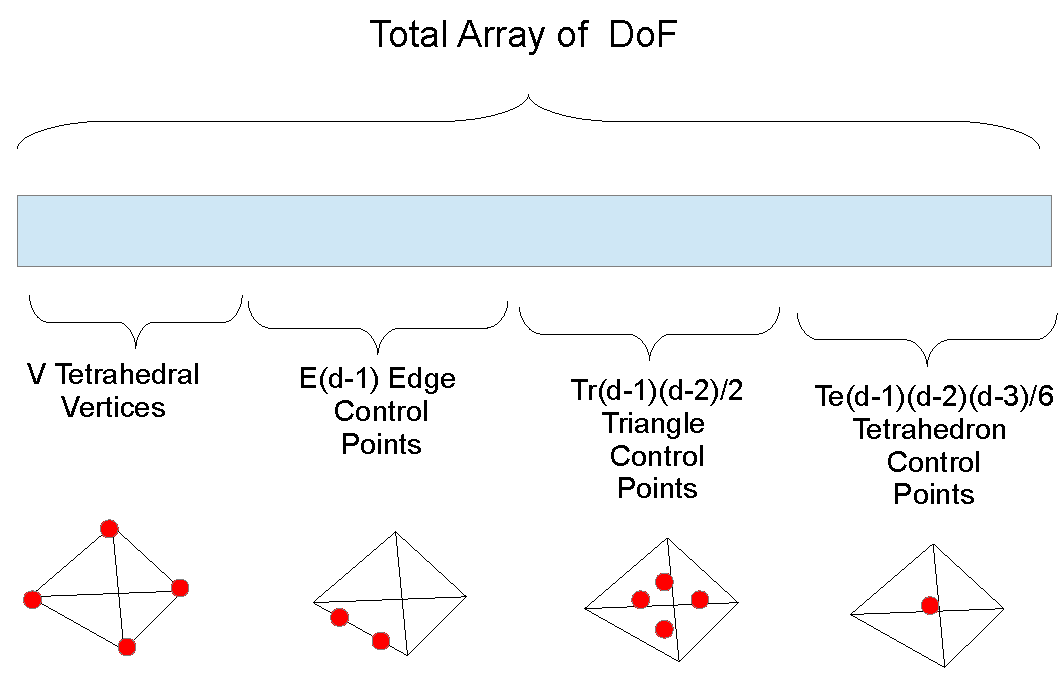
\includegraphics[width=0.80\textwidth]{DofLayoutBezierTetrahedron}
	\caption{Layout of Degrees of Freedom of Bezier Tetrahedral meshes inside a MechanicalState object}
	\label{fig:LayoutBezierTetrahedron}
\end{figure}

There are however some issues. In a tetrahedral mesh, edges and triangles are not oriented ({\em e.g.} a triangle is common to 2 tetrahedra and is ordered differently among each tetrahedron) and therefore the order in the DoF array may not reflect the order in each tetrahedron. It is the role of the BezierTetrahedronSetTopologyContainer class to provide a proper ordering.

Second, since there are several control points for a given edge, triangle and tetrahedron, it is important to specify the ordering inside each element. Figure\ref{DofBezierTetrahedronTesselation}

\begin{figure}[!htbp]
	\centering
    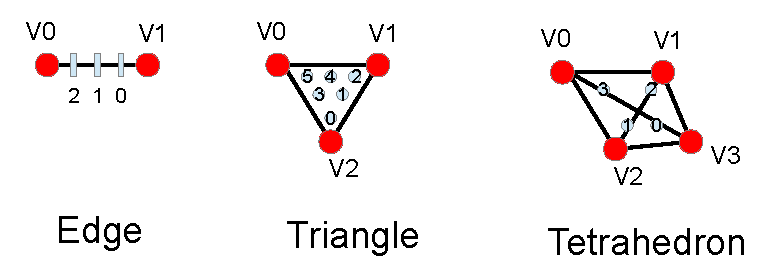
\includegraphics[width=0.80\textwidth]{DofBezierTetrahedronTesselation}
	\caption{Layout of Degrees of Freedom of Bezier Tetrahedral meshes inside a MechanicalState object}
	\label{fig:LayoutBezierTetrahedron}
\end{figure}

\subsection{BezierTetrahedronSetTopologyContainer Class}

This class describes 

\subsection{BezierTetrahedronSetGeometryAlgorithms Class}

\end{document}          

